\section{Análise e Discussão dos Resultados}
\label{sec:resultados}

Esta seção apresenta os resultados obtidos com a aplicação dos dois estágios descritos na metodologia e os discute à luz da literatura. Inicialmente, caracterizam-se o contexto socioeconômico e educacional do Maranhão e a distribuição do IDEB entre os municípios, o que evidencia a variabilidade de desempenho que motiva a investigação. Em seguida, responde-se à QP1, com a segmentação socioeconômica obtida com o \textit{K-Means}, e à QP2, com os fatores que diferenciam os municípios de alto e de baixo desempenho dentro de cada grupo com amostra suficiente. Por fim, esses achados são confrontados com a literatura e traduzidos em implicações para as políticas educacionais.

\subsection{Contexto socioeconômico e educacional do Maranhão}

O Maranhão é o segundo maior estado do Nordeste em extensão territorial e um dos mais populosos, com 217 municípios distribuídos em cinco mesorregiões. No Censo Demográfico 2022, o estado tem a menor renda domiciliar \textit{per capita} entre as 27 unidades da federação (R\$~899,87, contra R\$~1.638,06 no Brasil) \citep{ibge2022}. Tem também a segunda maior proporção de moradores em pobreza extrema, isto é, com rendimento \textit{per capita} de até 1/4 do salário mínimo ou sem rendimento (26,6\%, contra 13,3\% no Brasil) \citep{ibge2022classes}. Entre os municípios, a desigualdade também é expressiva: a renda \textit{per capita} mediana é de R\$~667, e a proporção de moradores em pobreza extrema varia de 11,2\% a 60,3\%. Esse contexto reflete-se nos resultados educacionais.

A Figura~\ref{fig:dist_ideb} apresenta a distribuição do IDEB dos 216 municípios com indicador divulgado. A distribuição é aproximadamente unimodal, ligeiramente assimétrica à direita, com média de 5,39 (desvio-padrão de 0,59), mediana de 5,30, mínimo de 4,10 e máximo de 8,10. A cauda superior é rarefeita: apenas 11 municípios atingem 6,50, e o máximo de 8,10 está um ponto acima do segundo maior valor (7,10).

\begin{figure}[!ht]
    \centering
    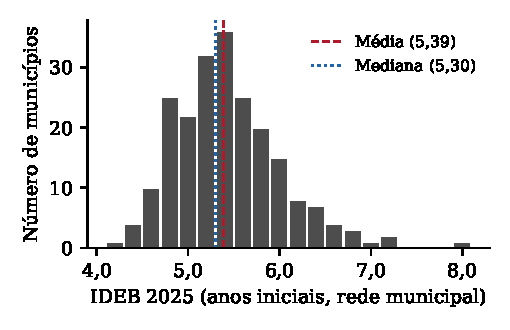
\includegraphics[width=\linewidth]{distribuicao_ideb.pdf}
    \caption{Distribuição do IDEB 2025 dos 216 municípios maranhenses com indicador divulgado (rede municipal, anos iniciais do ensino fundamental), em classes de 0,2 ponto. As linhas verticais marcam a média (5,39) e a mediana (5,30). Fonte: elaboração própria com dados de \citet{inep2025}.}
    \label{fig:dist_ideb}
\end{figure}

A amplitude de 4,00 pontos (4,10 a 8,10) é expressiva, dado que o IDEB varia de 0 a 10. Isso indica que, mesmo dentro do Maranhão, estado homogeneamente vulnerável em termos nacionais, existe variabilidade interna substancial, o que justifica investigar os fatores associados aos destaques positivos. Responder a essa pergunta exige, primeiro, reduzir a influência do contexto por meio de uma segmentação explícita e, depois, comparar, dentro de cada grupo, os municípios de alto e baixo desempenho.

\subsection{QP1: segmentação socioeconômica dos municípios}

A clusterização \textit{K-Means} foi aplicada sobre a \textit{renda per capita} e a \textit{pobreza extrema} (padronizadas pela mediana e pelo intervalo interquartil), testando de 2 a 10 grupos, conforme descrito na metodologia.

A Figura~\ref{fig:elbow} apresenta as curvas de inércia (cotovelo) e de \textit{Silhouette Score}. O \textit{Silhouette Score} atinge o valor máximo em $k = 3$ (0,506), acima de $k = 2$ (0,489) e de $k = 4$ (0,456). A estabilidade \textit{bootstrap} confirma a escolha: o ARI médio é 0,812 em $k = 3$, contra 0,744 em $k = 2$ e 0,704 em $k = 4$. Os dois critérios apontam, portanto, para a mesma partição, que é ao mesmo tempo a mais bem separada e a mais estável sob reamostragem entre as testadas. A curva de inércia decresce de forma gradual e não oferece, por si só, um critério adicional.

\begin{figure*}[!ht]
    \centering
    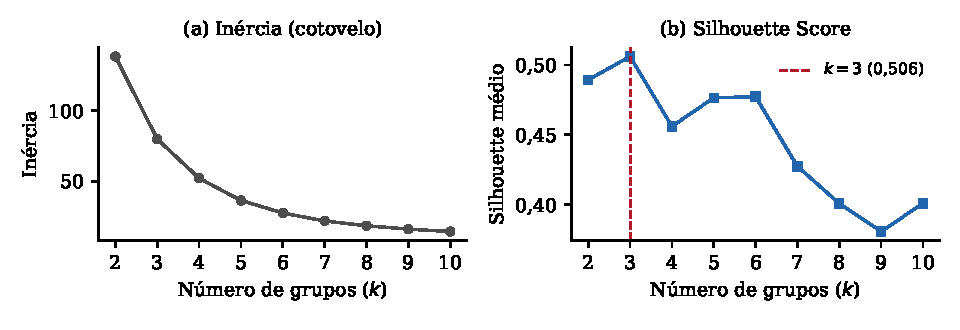
\includegraphics[width=0.85\linewidth]{elbow_silhouette.pdf}
    \caption{Escolha do número de \textit{clusters} para $k \in \{2, \ldots, 10\}$: (a) inércia intragrupo (Método do Cotovelo); (b) \textit{Silhouette Score} médio, com o máximo em $k = 3$ (0,506) marcado pela linha tracejada. Fonte: elaboração própria com dados de \citet{ibge2022, ibge2022classes}.}
    \label{fig:elbow}
\end{figure*}

A Figura~\ref{fig:pca} exibe os \textit{clusters} projetados nas duas primeiras componentes principais (a primeira componente, PC1, explica 93,6\% da variância; a segunda, PC2, explica 6,4\%). A predominância da primeira componente reflete a correlação entre as duas variáveis de segmentação: os municípios se distribuem essencialmente ao longo de um eixo de renda, no qual renda média alta e pobreza extrema baixa caminham juntas, e os três \textit{clusters} ocupam faixas sucessivas desse eixo.

\begin{figure}[!ht]
    \centering
    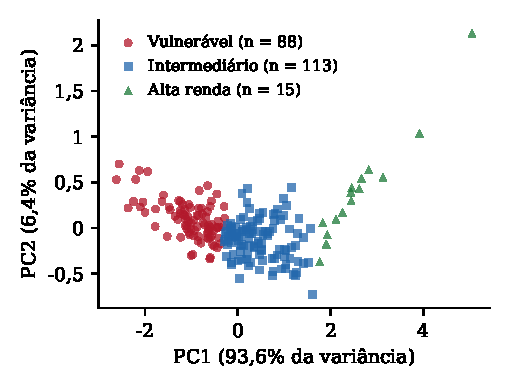
\includegraphics[width=\linewidth]{pca_clusters.pdf}
    \caption{Projeção dos 216 municípios maranhenses nas duas primeiras componentes principais, por \textit{cluster} socioeconômico ($k = 3$). Cada \textit{cluster} tem cor e marcador próprios. O eixo horizontal (PC1) concentra quase toda a variância e ordena os municípios da maior para a menor vulnerabilidade, da esquerda para a direita. Fonte: elaboração própria com dados de \citet{ibge2022, ibge2022classes}.}
    \label{fig:pca}
\end{figure}

O teste de ablação indica que as duas variáveis contribuem para a partição, com peso maior para a renda média. Refazendo a clusterização sem a renda \textit{per capita}, a concordância com a partição original cai para um ARI de 0,379; sem a pobreza extrema, o ARI é de 0,688. A pobreza extrema, portanto, não é redundante: a retirada dessa variável reclassifica parte relevante dos municípios, o que confirma que ela acrescenta à renda média a informação sobre a base da distribuição de renda.

A Tabela~\ref{tab:clusters} resume os três \textit{clusters} obtidos, denominados pelo critério de renda média. O \textit{cluster} de alta renda reúne a capital e os principais polos regionais do estado: São Luís, São José de Ribamar, Paço do Lumiar, Imperatriz, Timon, Açailândia, Balsas, Santa Inês, Pedreiras, Presidente Dutra, Porto Franco, Estreito, Carolina, Fortaleza dos Nogueiras e Itinga do Maranhão.

\begin{table}[!ht]
    \caption{Perfil dos \textit{clusters} socioeconômicos (médias municipais). Fonte dos dados: \citet{ibge2022, ibge2022classes, inep2025, inep2026microdados, inep2026sinopse}; cálculos próprios.}
    \label{tab:clusters}
    \centering
    \begin{tblr}{%
        colspec = {X[l] r r r},
        cells   = {font=\small},
        row{1}  = {font=\small\bfseries},
        width   = \linewidth
        }
        \toprule
        Indicador & Vulnerável & Intermediário & Alta renda \\
        \midrule
        Municípios (n) & 88 & 113 & 15 \\
        Renda \textit{per capita} (R\$) & 555,84 & 732,06 & 1.082,44 \\
        Pobreza extrema (\%) & 41,8 & 27,5 & 15,3 \\
        IDEB 2025 & 5,29 & 5,42 & 5,78 \\
        Escolas com internet (\%) & 83,8 & 89,0 & 94,3 \\
        Escolas com biblioteca ou sala de leitura (\%) & 15,8 & 19,3 & 38,7 \\
        Docentes EFAI com ensino superior (\%) & 55,9 & 64,0 & 79,1 \\
        \bottomrule
    \end{tblr}
\end{table}

O \textit{cluster} de alta renda, com 15 municípios, não tem amostra suficiente para a análise intragrupo por quartis, que resultaria em quatro ou cinco municípios em cada extremo. A análise comparativa é, portanto, conduzida nos \textit{clusters} vulnerável e intermediário, que juntos reúnem 201 dos 216 municípios analisados.

Os percentuais médios das variáveis de infraestrutura e de formação docente acompanham o gradiente de renda. A \textit{conectividade à internet} cresce de 83,8\% das escolas municipais no \textit{cluster} vulnerável para 94,3\% no de alta renda. O acesso a \textit{biblioteca ou sala de leitura} é baixo nos dois primeiros grupos e mais que dobra no de alta renda. A proporção média de \textit{docentes EFAI com ensino superior} vai de 55,9\% a 79,1\%, diferença que antecipa uma das hipóteses testadas no estágio intragrupo. Em resposta à QP1, os municípios maranhenses se organizam em três \textit{clusters} socioeconômicos ordenados pela renda, em uma partição estável sob reamostragem para a qual as duas variáveis contribuem.

\subsection{QP2: fatores discriminantes dentro dos \textit{clusters}}

A Tabela~\ref{tab:mw} reúne as variáveis com $p < 0{,}10$ no teste de Mann-Whitney nos dois \textit{clusters} analisados; as diferenças entre proporções são expressas em pontos percentuais (p.p.).

\begin{table*}[!ht]
    \caption{Variáveis com diferença entre municípios de alto e de baixo IDEB nos \textit{clusters} vulnerável e intermediário (Mann-Whitney bicaudal, $p < 0{,}10$). Alto e Baixo: médias dos grupos de alto e de baixo IDEB; $\Delta$: diferença entre as médias; $U$: estatística de Mann-Whitney; $\delta$: delta de Cliff; $q$: valor $q$ de Benjamini-Hochberg sobre as catorze variáveis de cada \textit{cluster}. Fonte dos dados: \citet{inep2026microdados, inep2025, inep2026sinopse, ibge2022, ibge2022classes}; cálculos próprios em Python (SciPy).}
    \label{tab:mw}
    \centering
    \begin{tblr}{%
        colspec = {X[l] r r r r r r r},
        cells   = {font=\small},
        row{1}  = {font=\small\bfseries},
        width   = 0.92\linewidth
        }
        \toprule
        Variável & Alto & Baixo & $\boldsymbol{\Delta}$ & $\boldsymbol{U}$ & $\boldsymbol{\delta}$ & $\boldsymbol{p}$ & $\boldsymbol{q}$ \\
        \midrule
        \SetCell[c=8]{l}{\textit{Cluster vulnerável (alto: n = 24; baixo: n = 23)}} & & & & & & & \\
        Docentes com ensino superior (\%) & 60,6 & 49,0 & $+$11,6 p.p. & 373,5 & 0,35 & 0,039 & 0,34 \\
        Docentes com licenciatura (\%)    & 59,1 & 47,8 & $+$11,4 p.p. & 369,0 & 0,34 & 0,049 & 0,34 \\
        \midrule
        \SetCell[c=8]{l}{\textit{Cluster intermediário (alto: n = 34; baixo: n = 29)}} & & & & & & & \\
        Escolas com quadra esportiva (\%)             & 12,9 & 5,4  & $+$7,5 p.p.  & 699,5 & 0,42 & 0,004 & 0,052 \\
        Turmas de correção de fluxo, anos finais (\%) & 0,90 & 0,07 & $+$0,8 p.p.  & 622,0 & 0,26 & 0,007 & 0,052 \\
        Docentes com ensino superior (\%)             & 69,2 & 58,1 & $+$11,1 p.p. & 637,5 & 0,29 & 0,047 & 0,18 \\
        Docentes com licenciatura (\%)                & 67,4 & 57,4 & $+$10,1 p.p. & 635,0 & 0,29 & 0,051 & 0,18 \\
        Renda \textit{per capita} (R\$)               & 753,15 & 719,13 & $+$34,02 & 620,0 & 0,26 & 0,081 & 0,23 \\
        \bottomrule
    \end{tblr}
\end{table*}

\subsubsection{\textit{Cluster} vulnerável}

Dentro do \textit{cluster} vulnerável (n = 88), os 24 municípios que se encontram no quartil superior de IDEB (alto, $\geq 5{,}60$, média 6,08) são comparados aos 23 do quartil inferior (baixo, $\leq 4{,}80$, média 4,61). A diferença média de 1,47 ponto de IDEB entre os grupos é substancial: equivale a quase dois desvios-padrão e meio da distribuição estadual.

A formação docente é a única dimensão que diferencia os municípios de alto e baixo IDEB no \textit{cluster} vulnerável. Os municípios de IDEB alto têm, em média, 11,6 p.p. a mais de \textit{docentes com ensino superior} e 11,4 p.p. a mais com \textit{licenciatura}, diferenças de efeito médio ($\delta$ de 0,35 e 0,34). Isoladamente, porém, esses testes não resistem à correção para comparações múltiplas ($q = 0{,}34$). A correlação de Spearman com todos os 88 municípios do \textit{cluster}, sem o descarte do intervalo central, confirma a associação com mais força: $\rho = 0{,}29$ para docentes com ensino superior ($p = 0{,}007$; $q = 0{,}063$) e $\rho = 0{,}28$ para licenciatura ($p = 0{,}009$; $q = 0{,}063$). Nenhuma outra variável mantém associação com o IDEB no \textit{cluster} após a correção ($q > 0{,}40$ em todas). Com a formação docente medida apenas na rede municipal, a associação se mantém e fica mais forte ($\delta$ de 0,38 e 0,42; $\rho$ de 0,32 e 0,35; $p \leq 0{,}026$), o que indica que a inclusão de docentes de outras redes na Sinopse não explica o resultado.

As duas variáveis se sobrepõem em grande parte (quase todos os docentes com ensino superior são licenciados) e devem ser lidas como um único achado. Ele dialoga com a literatura sobre o papel do professor \citep{rivkin2005} e com a meta nacional de formação em licenciatura \citep{brasil2014}, mas mede titulação, e não qualidade docente, e o faz no agregado municipal. \citet{rivkin2005} analisaram professores e alunos e encontraram pouca relação entre a titulação e o aprendizado, e a revisão de \citet{glewwe2013} chega a conclusão semelhante para países em desenvolvimento, nos estudos de maior rigor metodológico. Uma leitura possível é que, em redes nas quais mais de 40\% dos docentes ainda não concluíram a graduação, como as do \textit{cluster} vulnerável, a titulação diferencie os municípios mais do que em contextos em que ela já é quase universal.

A renda \textit{per capita} e a pobreza extrema não diferenciam os grupos de alto e baixo IDEB dentro desse \textit{cluster} ($p = 0{,}322$ e $p = 0{,}463$). Esse resultado é compatível com o propósito da segmentação: dentro do grupo, não se detecta diferença de renda entre os municípios de alto e de baixo IDEB. A ausência de significância, porém, não demonstra equivalência, sobretudo com grupos de 23 e 24 municípios, e diferenças socioeconômicas não captadas pela renda podem persistir.

\subsubsection{\textit{Cluster} intermediário}

Dentro do \textit{cluster} intermediário (n = 113), os 34 municípios do quartil superior de IDEB (alto, $\geq 5{,}70$, média 6,07) são comparados aos 29 do quartil inferior (baixo, $\leq 5{,}00$, média 4,81).

A formação docente reaparece no \textit{cluster} intermediário com magnitude semelhante à observada entre os municípios vulneráveis: 11,1 p.p. a mais de \textit{docentes com ensino superior} e 10,1 p.p. a mais com \textit{licenciatura} nos municípios de IDEB alto, com efeito médio ($\delta = 0{,}29$). A correlação de Spearman com todos os 113 municípios aponta na mesma direção ($\rho = 0{,}21$ e $0{,}20$; $p = 0{,}027$ e $0{,}036$), embora sem resistir à correção ($q$ de 0,12 e 0,13). A medida restrita à rede municipal reproduz o resultado com efeitos maiores ($\delta$ de 0,38 e 0,35; $p \leq 0{,}018$). Nenhum desses testes, isoladamente, é conclusivo; o que sustenta o achado é a sua repetição, com a mesma direção e magnitude, em dois grupos socioeconômicos distintos e nos dois procedimentos de comparação. Isso sugere que a associação entre formação docente e desempenho não se restringe a um único contexto socioeconômico.

A \textit{quadra esportiva} apresenta a diferença mais expressiva do \textit{cluster} ($p = 0{,}004$; $q = 0{,}052$; $\delta = 0{,}42$): as escolas com quadra são mais que o dobro nos municípios de IDEB alto (12,9\% contra 5,4\%), e a associação se mantém com todos os municípios do \textit{cluster} ($\rho = 0{,}23$; $q = 0{,}090$). Como a medida é municipal, o resultado não indica um efeito da atividade esportiva sobre os alunos. A presença de quadras pode sinalizar um padrão mais amplo de investimento da rede em infraestrutura escolar, leitura compatível com estudos que associam a infraestrutura ao IDEB, sobretudo nos anos iniciais \citep{alves2013, vasconcelos2021}; a análise, porém, não permite distinguir entre essas leituras. A proporção de turmas de correção de fluxo nos anos finais também é maior nos municípios de IDEB alto ($p = 0{,}007$; $q = 0{,}052$), mas os valores são pequenos (menos de 1\% das turmas), o efeito é pequeno ($\delta = 0{,}26$), e o resultado não permite inferir se a oferta de correção de fluxo é causa ou consequência do desempenho.

Diferentemente do \textit{cluster} vulnerável, a renda \textit{per capita} ainda apresenta diferença marginal entre os grupos ($p = 0{,}081$), de R\$~34 em média, o que indica alguma heterogeneidade residual de renda no \textit{cluster} intermediário, o maior dos três.

\subsubsection{Poder preditivo das variáveis}

As diferenças identificadas nos extremos de desempenho não se traduzem em capacidade de previsão. Em validação cruzada, o classificador \textit{Random Forest} não separou os municípios de alto e de baixo IDEB melhor que o acaso (AUC de 0,51 no \textit{cluster} vulnerável e de 0,57 no intermediário). A regressão \textit{ridge} não previu o IDEB melhor que a média, nem no estado como um todo ($R^2 = -0{,}01$), nem dentro dos \textit{clusters} ($R^2$ de $-0{,}10$ e $-0{,}07$). Os fatores discriminantes descritos acima são, portanto, associações específicas e de magnitude modesta: a maior parte da variação do IDEB entre municípios depende de fatores que as variáveis administrativas disponíveis não captam.

Em resposta à QP2, a formação docente é o fator que diferencia os municípios de alto e de baixo IDEB nos dois \textit{clusters} analisados, com efeito médio e de forma consistente entre procedimentos; no \textit{cluster} intermediário, somam-se a quadra esportiva e, com efeito pequeno, a correção de fluxo. Nenhum desses fatores, isoladamente ou em conjunto, prevê o desempenho.

\subsection{Diálogo com a literatura}

Os achados dialogam com a literatura de maneiras específicas. A centralidade da qualificação docente, observada nos dois \textit{clusters} com diferenças de 10 a 12 p.p. entre municípios de alto e baixo IDEB, é compatível com a ênfase da literatura no papel do professor \citep{rivkin2005} e com a prioridade que a política nacional atribui à formação em licenciatura \citep{brasil2014, gatti2019}. Vale a ressalva já apontada: o estudo mede a titulação no agregado das redes municipais, e não a qualidade de cada docente. A pesquisa em eficácia escolar \citep{brooke2008} oferece o enquadramento para esse resultado: controlado o contexto socioeconômico, parte da diferença de desempenho entre redes se associa a características das próprias redes escolares. A ausência de diferença significativa de renda e de pobreza extrema dentro do \textit{cluster} vulnerável é consistente com a tese de \citet{coleman1966} de que o contexto socioeconômico explica a maior parte da variação do desempenho. Quando esse contexto é aproximadamente controlado, as diferenças que restam passam a se associar a fatores escolares, de magnitude menor.

Em relação à literatura de mineração de dados educacionais, o trabalho contribui com uma aplicação metodológica que responde a duas limitações apontadas na Seção~\ref{sec:relacionados}: o uso de modelos globais que ignoram a heterogeneidade socioeconômica entre municípios e a menor presença de estudos sobre o Norte e o Nordeste. Em vez de produzir perfis como resultado final \citep{alves2014}, o agrupamento definiu os grupos de comparação do segundo estágio, e a validação da partição por \textit{Silhouette}, estabilidade e ablação dá transparência a essa etapa. A abordagem em dois estágios é replicável para outros estados e pode ser adaptada a outros níveis de ensino (anos finais do ensino fundamental, ensino médio) ou a outras medidas de desempenho. O baixo poder preditivo, por sua vez, é um resultado relevante para a área: modelos supervisionados treinados apenas com variáveis do Censo Escolar dificilmente separarão redes de alto e de baixo desempenho dentro de um mesmo contexto socioeconômico.

Quanto ao IDEB como métrica, os pressupostos estatísticos identificados por \citet{soares2013}, especialmente a correlação entre fluxo e proficiência, não invalidam a análise, mas sugerem cautela na interpretação: municípios com IDEB elevado podem estar priorizando aprovação em detrimento da proficiência. A inclusão de variáveis de fluxo (\textit{distorção idade-série}, \textit{correção de fluxo}) entre as explicativas não elimina esse risco: como o próprio IDEB incorpora a taxa de aprovação, essas variáveis guardam relação parcialmente mecânica com a variável-alvo, e as diferenças observadas nelas devem ser lidas com essa ressalva.

\subsection{Implicações para as políticas educacionais}

Os resultados têm implicações para gestores municipais e formuladores de políticas educacionais do Maranhão:

\begin{itemize}
  \item \textbf{Formação e habilitação docente (\textit{clusters} vulnerável e intermediário).} A diferença de 10 a 12 p.p. na proporção de \textit{docentes com ensino superior} entre municípios de alto e baixo IDEB se repete nos dois grupos analisados. Isso torna programas de formação continuada e de indução à licenciatura específica candidatos plausíveis de política pública em todo o estado, e não apenas nos municípios mais pobres. A análise associativa não permite, porém, quantificar o impacto esperado. Políticas de financiamento de graduação para docentes em exercício, como o Programa Nacional de Formação de Professores da Educação Básica (Parfor), são instrumentos já existentes cuja ampliação pode ser considerada, com avaliação de impacto que confirme o efeito sobre o desempenho.

  \item \textbf{Infraestrutura escolar (\textit{cluster} intermediário).} A quadra esportiva ($p = 0{,}004$; $q = 0{,}052$; $\delta = 0{,}42$) destaca-se como fator discriminante nos municípios de renda intermediária, sugerindo que, nesse grupo, o investimento em infraestrutura física complementar é candidato a priorização no monitoramento e na alocação orçamentária, ainda que a análise não permita estimar o retorno esperado desse investimento.

  \item \textbf{Monitoramento por perfil socioeconômico.} A segmentação permite que as redes se comparem com municípios de contexto semelhante, e não com médias estaduais ou nacionais. Municípios de IDEB alto dentro de cada \textit{cluster} podem servir de referência para os demais do mesmo grupo.
\end{itemize}
